\subsection{Efficiency and Kill Rates}

At 0\% luck and SR settings, the game is $\textbf{deterministic}$. 1.8 becomes 2, 2.4 becomes 2, 3.2 becomes 3, and so on. The result of any battle is 100\% predictable once you know the stack sizes. The vast majority of templates use the 60/70 kill rate ratio which introduces just enough variety and strategy to make things competitive. At lower attack rates, big bonuses are painfully slow and you favour dense, high-income region instead. At higher defender rate, attrition is increased. Each extra income saves you more over time. At the 60/70 rates, the break-even ratio floats around 1.7, meaning you need generally around 1.7 more attackers than defenders, while at something like 30/40, that ratio jumps to 2.3-2.5, effectively meaning a small income swing no longer guarantees you'll ever cross the line and stalemates occur more easily. But what does it mean behind the scenes. 
\\
\\
With 0\% luck and SR settings, the armies you kill are $Kills = \text{round}(p \times N)$ where, 
\begin{itemize}
    \item $p=0.60$ for attackers or 0.70 for defenders
    \item round means nearest integer. 0.5 rounds up.
\end{itemize}
If we write p as a reduced fraction:
\begin{itemize}
    \item $p = 3/5$ (attack) -> denominator 5 -> five distinct curves
    \item $p = 7/10$ (defense) -> denominator 10 -> ten curves
\end{itemize}
Let $N = dk + r$ for d the denominator (5 or 10) and r its remainder.
\begin{itemize}
    \item Attacker kills $K = 3\times k + \text{round}(3 \times r / 5)$
    \item Efficiency given as $K/N = (3/5) + \delta / N$ for $\delta$ in the range $[-0.5, +0.5]$
    \item As N, the number of attacker, grows, $\delta / N$ approaches 0, so every curve asymptotically tends to 0.60 (or 0.70).
\end{itemize}
In other words, small attacks are always more efficient than big attacks. But also some attacks are generally more efficient than others from the above 5/10 distinct curves.

\subsubsection{Attacker Curves at p = 0.60}

%----------------- 1. Attacker residue curves (p = 0.60) -----------------
\small
\begin{longtable}{|c|l|c|c|l|}
\hline
\rowcolor{Baby_Blue}
Residue $r$ (mod 5) & Sequence ($N$) & round$(3r/5)$ & First Kills / $N$ & Behaviour \\ 
\hline\hline
\endfirsthead
\hline
\rowcolor{Baby_Blue}
Residue $r$ (mod 5) & Sequence ($N$) & round$(3r/5)$ & First Kills / $N$ & Behaviour \\ 
\hline\hline
\endhead
0 & $5,10,15,\dots$ & 0 & 60\% & Flat at 60\% (perfect multiples) \\ \hline
1 & $1,6,11,16,\dots$ & 1 & 100\%, 66.7\%, \dots & Starts above 60\%, then falls \\ \hline
2 & $2,7,12,17,\dots$ & 1 & 50\%, 57.1\%, \dots & Starts below 60\%, then rises \\ \hline
3 & $3,8,13,18,\dots$ & 2 & 66.7\%, 62.5\%, \dots & Starts above 60\%, then falls \\ \hline
4 & $4,9,14,19,\dots$ & 2 & 50\%, 55.6\%, \dots & Starts below 60\%, then rises \\ \hline
\caption{Attacker efficiency curves ($p = 0.60$) under 0\,\% Luck + Straight Round}
\label{table:attackerResidue}
\end{longtable}
\normalsize

To elaborate.
\begin{itemize}
    \item Multiples of 5 are never wrong. Perfectly on-rate and easy to memorize, always kill 60\%.
    \item The bigger the attack, the less efficient it is. Take residue of 1 at mod 5, the most efficient attacks. An attack of 1 army guarantees you a 1:1 exchange. An attack of 6 kills 0.66, an attack of 11 0.63, an attack of 16 0.625 and so on till it reaches asymptotically the 0.60 attackers kill rate.
\end{itemize}
Attacks at residue 0,1 or 3, are generally a lot more efficient than residue 2 and 4. This is a very complex way of describing why you send attack with 3 instead of 4 attackers. 6 instead of 7, and so on. Same kills, fewer losses, more efficient. Sequences at 1 or 3 give you the best per-army punch when stacks are small, but once you bypass approximately 20 troops, the edge shrinks below 1\%, and "just send what you've got" is fine.

\subsubsection{Defender Curves at p = 0.70}

%----------------- 2. Defender residue curves (p = 0.70) -----------------
\small
\begin{longtable}{|c|c|l|c|l|}
\hline
\rowcolor{Baby_Blue}
$r$ (mod 10) & round$(7r/10)$ & Sequence ($N$) & First Kills / $N$ & Behaviour \\ 
\hline\hline
\endfirsthead
\hline
\rowcolor{Baby_Blue}
$r$ (mod 10) & round$(7r/10)$ & Sequence ($N$) & First Kills / $N$ & Behaviour \\ 
\hline\hline
\endhead
0 & 0 & $10,20,\dots$ & 70\% & Flat at 70\% (multiples of 10) \\ \hline
1 & 1 & $1,11,21,\dots$ & 100\%, 72.7\%, \dots & Starts high, then falls \\ \hline
2 & 1 & $2,12,22,\dots$ & 50\%, 66.7\%, \dots & Starts low, then rises \\ \hline
3 & 2 & $3,13,23,\dots$ & 66.7\%, 69.2\%, \dots & Starts low, then rises \\ \hline
4 & 3 & $4,14,24,\dots$ & 75\%, 71.4\%, \dots & Starts high, then falls \\ \hline
5 & 4 & $5,15,25,\dots$ & 80\%, 76\%, \dots & Peaks at 80\%, then falls \\ \hline
6 & 4 & $6,16,26,\dots$ & 66.7\%, 68.8\%, \dots & Starts low, then rises \\ \hline
7 & 5 & $7,17,27,\dots$ & 71.4\%, 70.6\%, \dots & Starts high, then falls \\ \hline
8 & 6 & $8,18,28,\dots$ & 75\%, 72.2\%, \dots & Starts high, then falls \\ \hline
9 & 6 & $9,19,29,\dots$ & 66.7\%, 68.3\%, \dots & Starts low, then rises \\ \hline
\caption{Defender efficiency curves ($p = 0.70$) under 0\,\% Luck + Straight Round}
\label{table:defenderResidue}
\end{longtable}
\normalsize

After approximately 30\% defenders, every curve is within $\pm 1\%$ of 0.70. The same mathematical logic applies here as well. Take for example r 1. 11 defenders kill 0.727, 21 defenders kill 0.714, 31 defenders kill 0.709 and so on approaching asymptotically 0.70. Some r's approach 0.7 from higher values, some from lower values. The biggest take away you can get from the table is to never end a turn defending a territory on 2,3,6,9 etc. Well, almost never. There can always be very specific scenarios where this would do the trick but it generally leads to losses of armies. 5-defender blocks are outright the most efficient thing you can do. 

\subsubsection{Practical tips}

All this gets highly mathematical but there's a lot of takeaways and you have to keep in mind every thing here is very case-specific. Doing exclusively attacks of 1 and 6 won't win you every game.
\begin{itemize}
    \item Using 3-, 6-, 11- attacks are the most efficient. These numbers sit on the |66\% starts-high| attacker curve and kill as many as 4/7/8 would but cost one fewer unit every single swing. 
    \item Defending with 2,3,6,9 etc is inefficient. This however doesn't mean it's always wrong. Yes, 6 defenders kill 4 attackers, as many as 5 defenders kill, yet they make the enemy jump from 8->10 attackers. This extra unit from the armies required from them can buy you an extra turn on a chokepoint. For example \href{https://www.warzone.com/MultiPlayer?GameID=39915640}{Turn 12, Greenland}. Though I still want to stress that ideas like these are useful to either make a comeback or provide a moveset for you that cannot go wrong. Generally you should think of efficiency as that will give you the necessary advantage in armies that can be converted to a win. Take into example this miserable \href{https://www.warzone.com/MultiPlayer?GameID=41012101}{Biomes} game I had once, and particularly turn 6 onwards. I need to play a crazy expansion game due to picking poorly and out of pure luck/my opponent misplaying it, I manage to get him to lose a card piece on turn 6 and transform the game into a 16v14 game (that becomes 12v11 after sanctions). However, do I have an advantage in reality? By end of turn 6, 
    \begin{enumerate}
        \item Syphen sure is down 1 income, but has a total of 14 movable armies, 10 in fronts, 4 delays.
        \item I (7ate9) have 9 movable armies. 6 in fronts and 3 delays.
    \end{enumerate}
    \item My income advantage is not seen, as I cannot realistically outdelay him, nor attack him due to having way less armies in our fronts. So I did the only thing I could do, play around efficient attacks/defenses and accept that I cannot do more, I need to have him throw armies in the bin to convert my advantage. And through an 8 army defense sit, and 2 attacks in USA of 3 and 6, just within one turn the movable armies in fronts went from 10v6 in his favor to 2v3 in my favor. While you shouldn't look into this as me making the perfect moves, you should get into the habit of investing time into every single move and idea you make in your game.
\end{itemize}

Information is power. As I stated in the beginning of this section, 0\% luck SR settings are deterministic. Deterministic combat turns this into a chess-like game where you enter lines, sequences of moves, based on how efficient you are. While you can keep as a rule of thumb which attacks and which defenses are the best, or tier them even, the ideas should pop in upon looking for forced moves. Take for example this \href{https://www.warzone.com/MultiPlayer?GameID=40190484}{Strat MME} game on Turn 4 at Figure \ref{finding_best_moves}.

\begin{figure}[H]
  \centering
  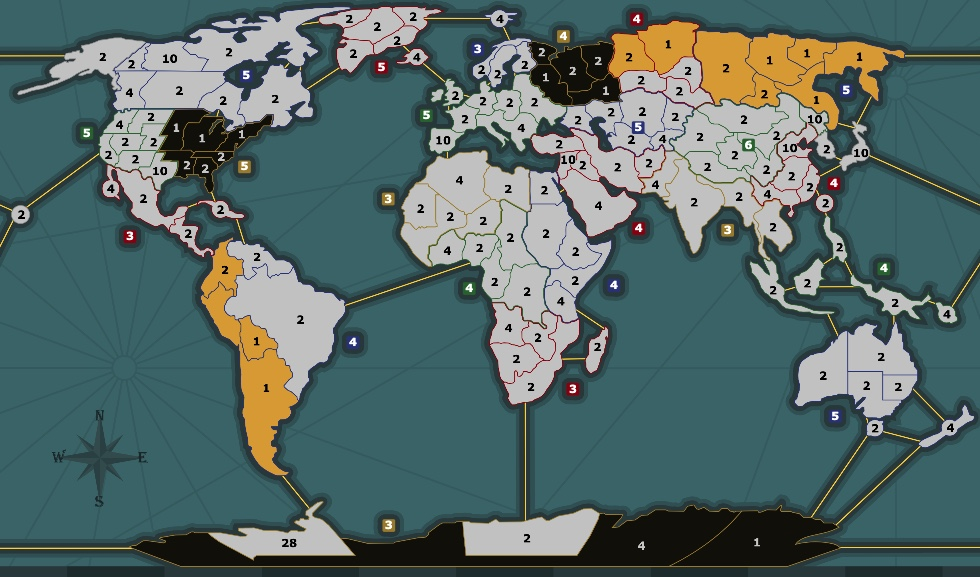
\includegraphics[width=0.7\textwidth]{Images/perf_moves.jpg}
  \caption{Finding Best Moves}
  \label{finding_best_moves}
\end{figure}

From Bast's perspective, you have information of all 3 enemy picks and you know the game is 14vs10 income and you know you have first move on the following turn. What do you do and what is your reasoning? Simplify the position, find moves that will work 100\% of the time. 
\begin{itemize}
    \item If you deploy +14 in Vorkuta and first move with 15, if Buns deploys +10, 16v12 becomes 7v3 and Buns can still coinflip break the other territory (the position is still completely winning for bast, it's a 10vs10 income game with $\sim$ 10 armies advantage). bast in this position can get the card piece in Antarctica.
    \item If you as bast think of the position as: "Buns has 10 income, he goes up to 12, kills up to 7, I can guarantee defense by deploying 6\&7, even 6\&6 and first move 1 extra army. I can force outdelay and then attack and slowly proceed". The end result isn't wrong, at the end of the turn Buns will likely get SA, and the game would now be a 14vs14 game with army advantage. The problem is that it's not a forced win and you waste armies in delays.
\end{itemize}
So we are stuck between these two ideas, or well, strategies. One of them is very safe and slow, the other risks a recapture of our bonus. Is it a prediction? No. Remember the kill rate tables and discussion. Why first move with 15vs12 instead of 13vs12? You can deploy +12 on Vorkuta and first move with 13, get at worse a trade of 14vs12 to 6vs4 and deploy the remaining 2 of your income in Ufa. Even if Buns decides to full deploy, his remaining alive defenders (3 after you subtract the army stand guard), cannot capture Ufa. 

\paragraph{Taps}

Tapping is an idea of attacking with exactly one army. Since $0.60 \times 1 = 0.60$ it rounds to 1, which is a perfect trade 1:1. The real value comes in specific scenarios, some of them explained later, but a crucial one the fact that taps change the remainder class of the enemy stack by -1, which can flip how the rounding behaves for a big attack the following turn. Practically speaking, lets define taps and their usage in 2 categories, offensively and defensively.

\begin{enumerate}
    \item Tapping as the attacker
    \begin{itemize}
        \item Useful for sniping leftover armies to deny delays
        \item Useful at reducing an opponent's stack through equal trades
        \item Useful at setting up a forced kill or sequence later on
    \end{itemize}
    \item Tapping as the defender
    \begin{itemize}
        \item Useful for sniping leftover armies to deny delays
        \item To gain a favourable kill rate. Table \ref{table:defenderTap}.
    \end{itemize}
\end{enumerate}

%----------------- Table 1 – Defender tap squeezes an extra army --------------
\scriptsize
\begin{longtable}{|c|c|c|c|}
\hline
\rowcolor{Baby_Blue}
Start (A v D) & Result if \textbf{attacker swings first} & Result if \textbf{defender taps, then attack} & Defender gains … \\ \hline\hline
\endfirsthead
\hline
\rowcolor{Baby_Blue}
Start (A v D) & No tap & Defender-tap line & Gain \\ \hline\hline
\endhead
6 v 6  & 2 v 3 & 1 v 3 & +1 net army \\ \hline
9 v 9  & 3 v 4 & 2 v 4 & +1 \\ \hline
12 v 12 & 4 v 5 & 3 v 5 & +1 \\ \hline
19 v 19 & 6 v 8 & 5 v 8 & +1 \\ \hline
\caption{One-army tap from the defender bumps the attacker into a worse rounding class; same casualties on the defender side, one extra loss for the attacker.}
\label{table:defenderTap}
\end{longtable}
\normalsize

In case this isn't self-explanatory, for example in the 9vs9 scenario:
\begin{itemize}
    \item No tap: 9vs9. 8 att kill 5. 9 defenders kill 6 -> 3vs4
    \item Yes tap: 9vs9-> 8vs8. 7 att kills 4. 8 defenders kill 6 -> 2vs4
\end{itemize}

The idea of sniping leftover armies to deny delays is something taking place predominantly in brawl templates, but can nonetheless be applied to everything. For example in this French Brawl  \href{https://www.warzone.com/MultiPlayer?GameID=21713173}{game} note how both players create artificial delays through tapping, on Turn 4 where Beep taps first order to reduce the opponent's stack, on Turn 5 where Othello taps a leftover south to deny from the opponent the extra delay they can gain from moving that, and so on. To expand on this idea, sometimes you need to first move attacks in order to deny from your opponent this 1:1 trade. For example in this French Brawl \href{https://www.warzone.com/MultiPlayer?GameID=41378170}{game} my opponent Turn 2 south should first move me with a 3attack, to get a better 2:1 trade for himself. Instead he allows me to get 2x 1:1 trades. This is practically risk-free when you have priority that turn, as in the opposite scenario your opponent might always move that army away and you get a 1:0 trade. For example in this French Brawl \href{https://www.warzone.com/MultiPlayer?GameID=40950869}{game} pay attention to Turn 2 where I tap on my first move (1:1 trade), and my opponent taps back the same territory (1:0 trade). Try to avoid these at all costs.
\\
\\

Min-maxing your armies through optimizing kill rates is almost a revolutionary concept to new players, and while it does take effort, it elevates your gameplay. It is, in my opinion, one of the three most important thing on your journey to becoming a better player, together with making great picks and understanding the template's and map's dynamics.